\documentclass[../../syllabus_2.tex]{subfiles}
\begin{document}

\chapter{Calcul littéral}

\faIcon{book} Théorie pages 136 à 140 et pages 157 à 158

\section{Rappels}

Une expression algébrique (ou expression littérale) est une expression dans laquelle se mêlent des nombres et des lettres. Chaque terme se compose d'un \textbf{coefficient} et d'une \textbf{partie littérale.}
\vspace*{0.5cm}
\begin{center}
  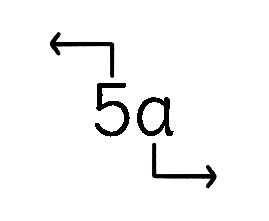
\includegraphics[width=3cm]{img/5a.pdf}
\end{center}

Notes~:
\begin{itemize}[label=$\bullet$, itemsep=0.5cm]
  \item $5a$ est l'écriture simplifiée de \dotfill
  \item Dans une expression littérale, on écrit toujours d'abord \dotfill\bigbreak et ensuite \dotfill
\end{itemize}

\begin{exercise}
  Calcule les valeurs numériques des expressions suivantes.
  \begin{enumerate} [cols=2]
    \item $2x+3x^2$ si $x=2$
    \item $-2+a-10ab$ si $a=3$ et $b=-1$
  \end{enumerate}
\end{exercise}

\newpage
\begin{enumerate}
  \adf[\item Dans une somme (ou une différence) algébrique, on ne peut réduire que ]{1}
\exemples
\begin{itemize}[cols=2, label=]
  \item $3a+2b-7a=$
  \item $13x - 7y + 10y - 3x=$
\end{itemize}

\vspace*{1cm}

\adf[\item Dans un produit algébrique, on multiplie]{1}
\exemples
\begin{itemize} [cols=2, label=]
  \item $-3a\cdot 6ab^3=$
  \item $5a\cdot (-7a^6)=$
\end{itemize}

\vspace*{1cm}

\adf[\item Pour effectuer une distributivité simple,]{1}
\exemples
\begin{itemize}[cols=2, label=]
  \item $2\left(5a+3\right)=$
  \item $3x\left(2xy - 5x\right)=$
\end{itemize}


\vspace*{1cm}

\adf[\item Pour mettre en évidence,]{3}
\exemples
\begin{itemize}[cols=2, label=]
  \item $2xy+4x=$
  \item $56a - 35a^2b=$
\end{itemize}

\end {enumerate} 


\newpage
\begin{exercise}
  Réduis au maximum les expressions suivantes.
  \begin{enumerate}[cols=2, itemsep=1cm]
    \item  $3a+2a=$
    \item  $5b+7=$
    \item  $3x \cdot 6xy=$
    \item  $3b+7a-2a+4b^3-a=$
    \item  $5(2x - 6)- 10 + (-5x)=$
    \item  $3a-2b+7a+12b=$
    \item  $10\left(4a+2\right)=$
    \item  $ax\left(x-2\right) -3x^2=$
    \item  $x+3xy-6y+3x=$
    \item  $2x^3 \cdot (2x^2)^3=$
  \end{enumerate}
\end{exercise}
\vspace*{1cm}

\begin{exercise}
  Transforme les sommes suivantes en produits, et inversément.
  nb: Soustraire une expression revient à ajouter son opposé.
  \vspace*{2cm}
  \begin{center}
    
    \begin{tblr}{hlines, vlines, columns={5cm,c},row{1}={c, font=\bfseries}, rowsep=1ex}
      \tikzmarknode{UL}{Somme}       & \tikzmarknode{UR}{Produit}               \\
       $6ab-12a$  &                       \\
                  & $2x\left(3-x\right)$  \\
                  & $10\left(a+2b\right)$ \\
      \tikzmarknode{BL}{$5x+20y$}    & \tikzmarknode{BR}{\phantom{$5x+20y$}}                      \\
    \end{tblr}
    \begin{tikzpicture}[remember picture, overlay, >=latex]
      \def\myspace{1.4ex}
      \draw[->] ($(UL.north)+(0,\myspace)$) to[out=45, in=135]node[above]{Factoriser} ($(UR.north) + (0,\myspace)$);
  
      \draw[<-] ($(BL.south)+(0,-\myspace)$) to[out=-45, in=-135]node[below]{Développer} ($(BR.south) + (0,-\myspace)$);
    \end{tikzpicture}
    
  \end{center}

\end{exercise}
\newpage
\section{Supprimer des parenthèses dans une somme algébrique}
Lorsqu'on souhaite simplifier l'écriture d'une somme algébrique, et donc enlever les parenthèses, deux cas de figures se présentent~:


 \adf[Si la parenthèse est précédée du signe \og$+$\fg\ (si on ajoute une parenthèse) :]{2}
  \exemples 
  \begin{itemize}[label=$\bullet$, cols=2]
    \item $3+\left(2-7\right)=$
    \item $27a+\left(10+3a\right)=$
  \end{itemize}

\vspace*{1cm}

\adf[Si la parenthèse est précédée du signe \og$-$\fg\ (si on retranche une parenthèse)~:]{2}
  \exemples 
  \begin{itemize}[label=$\bullet$, cols=2, itemsep=1.5cm]
    \item $3-\left(2-7\right)=$
    \item $27-\left(10+3\right)=$
    \item $2a-\left(a-7\right)=$
    \item $- (3a + 2x) + (-8x + a)=$
  \end{itemize}

\vspace*{1cm}

\textbf{Tableau de synthèse}

\begin{center} 
  \begin{tblr}{
  hlines, 
  vlines, 
  column{1}={5cm}, 
  column{2}={4cm},
  column{3}={5cm},
  rows={m},
  }
  S'il y a un "$\cdot$" devant ou derrière la (\dots)
  & $a\cdot(b+c) = ab + ac$
  & On effectue une distributivité simple.\\
  S'il y a un "$+$" devant la (\dots)
  & $a + (b-c) = a + b - c$
  & On enlève la (\dots) et rien ne change.\\
  S'il y a un "$-$" devant la (\dots) 
  & $a - (b-c) = a - b + c$
  & On distribue le "-" à chaque terme de la (\dots).\\
  \end{tblr}
\end{center}

\newpage
\begin{exercise}
  (Sur feuille annexe)  Réduis au maximum les expressions suivantes.
  \begin{enumerate}[cols=2]
    \item  $3x+\left(2-x\right)$
    \item  $17+13x+10\left(5x-3\right)$
    \item  $\left(3a+5\right) -17$
    \item  $6x-\left(3+5x\right)$
    \item  $1-\left(13+a-2b\right) + 3a - \left(2a-b\right)$
    \item $4x-3+2\left(5x-15\right)$
    \item $2a+\left(4a^2-5\right) - \left(2+3a^2\right)$
    \item $4x+\left(3x-6\right) -12$
    \item $2ab-3a+\left(5b-3\right)$
    \item $4xy+3x-2\left(2xy+3x\right) -17xy$
  \end{enumerate}
\end{exercise}

\newpage
\begin{exercise}
  Réduis les calculs suivants. Aide-toi de la résolution des deux premiers exemples. Si possible, réduis les fractions obtenues au maximum. \\
  \begin{enumerate}[cols=2, label=]
    \item 
    \textbf{Exemple 1}
    \medbreak
      $\begin{aligned}
      \dfrac{a}{3} - \dfrac{2+a}{3} 
      &= \dfrac{a}{3} - \dfrac{\left(2+a\right)}{3}\\
      &= \dfrac{a-\left(2+a\right)}{3}\\
      &= \dfrac{a-2-a}{3}\\
      &= \dfrac{-2}{3}
    \end{aligned}$
    \vspace{3cm}
    \item   
    \textbf{Exemple 2}
    \medbreak
      $\begin{aligned}
      \dfrac{a}{6} + \dfrac{2+a}{2} 
      &= \dfrac{a}{6} + \dfrac{3\left(2+a\right)}{6}\\
      &= \dfrac{a+6+3a}{6}\\
      &= \dfrac{6+4a}{6} \\
      &= \dfrac{2(3+2a)}{6}\\
      &= \dfrac{3+2a}{3} \\
    \end{aligned}$
  \end{enumerate}

  \begin{enumerate}[cols=2, itemsep=6cm]
    \item  $\dfrac{a}{4}-\dfrac{3+a}{4}=$
    \item  $\dfrac{c}{6} + \dfrac{3+c}{3}=$
    \item  $\dfrac{7+f}{5}-\dfrac{3f}{10}=$
    \item  $\dfrac{3(2p+2)}{8} - \dfrac{p+5}{2}=$
  \end{enumerate}
\end{exercise}

\vspace*{6cm}

\newpage
\section{Distributivité simple, distributivité double}
Nous connaissons déjà la distributivité simple, c'est-à-dire lorsque nous avons un facteur qui multiplie une somme de plusieurs termes qui se trouvent entre parenthèses.

\[a\left(b+c\right)=\]

Que se passe-t-il lorsque nous avons un produit où chacun des facteurs est une somme de deux ou plusieurs termes~?

\adf[Pour effectuer une distributivité double,]{2}

$\left(a+b\right)\left(c+d\right)=$
\vspace*{2cm}

\exemples \\
Avec les flèches :
\begin{itemize}[cols=2, label=, leftmargin=0pt]
  \item $\left(3x+5\right)\left(2-x\right)=$
  \item $\left(10a+3b-1\right)\left(2+3a\right)=$
\end{itemize}
\vspace*{2cm}

Avec la grille :
\begin{itemize}[cols=2,label=, leftmargin=0pt]
  \item $\left(3x+5\right)\left(2-x\right)=$
  \item $\left(10a+3b-1\right)\left(2+3a\right)=$
\end{itemize}
\vspace*{6cm}

\newpage
\begin{exercise}
  Développe et réduis au maximum.
  \begin{enumerate}[cols=2, itemsep=4cm]
    \item  $\left(x+1\right)\left(x+2\right)=$
    \item  $\left(2x+1\right)\left(3x-2\right)=$
    \item  $\left(2y+5\right)\cdot\left(1-4y\right)=$
    \item  $\left(2a+5\right)\left(3-a\right)=$
    \item  $\left(x+1\right)\left(x+2\right)-3\left(x-2\right)=$
    \item  $7x+\left(-6+x\right)\left(x+7\right)=$
    \item  $2\left(3x-1\right)=$
    \item  $\left(2x\right)^2-2\left(x+2\right)\left(x-3\right)=$
    \item  $3-\left(2+7a\right)-a=$
    \item  $2x\left(5x+5\right)-\left(2x-3\right)\left(1-x\right)=$
  \end{enumerate}
\end{exercise}

\newpage
\section{Produits remarquables}
Un produit remarquable est une technique plus rapide pour effectuer une double distributivité 
dans deux cas précis: le carré d'un binôme et le produit de binômes conjugués.

\vspace*{0.5cm}

\textbf{Un binôme} est une somme algébrique de deux termes. 

\subsection{Le carré d'une somme}

Formule du carré d'une somme :
\begin{equation*}
  \left(a+b\right)^2=a^2+2ab+b^2
\end{equation*}

\begin{spacing}{1.7}
Preuve : $
  \begin{aligned}[t]
    \left(a+b\right)^2
     & = \\
     & = \\
     & = \\
  \end{aligned}
$
\end{spacing}

\begin{exercise}
  Complète les développements ci-dessous.
  \begin{spacing}{2}
    \begin{enumerate}[itemsep=0.5cm]
      \item $
              \begin{aligned}[t]
                \left(2+x\right)^2 & = \left(\ldots \ldots\right)^2 + 2 \cdot  \ldots \ldots \cdot  \ldots \ldots + \left( \ldots \ldots\right)^2 \\
                                   & =  \ldots \ldots +  \ldots \ldots +  \ldots \ldots
              \end{aligned}
            $
      \item $
              \begin{aligned}[t]
                \left(3a+9\right)^2
                 & = \left( \ldots \ldots\right)^2 + 2 \cdot  \ldots \ldots \cdot  \ldots \ldots + \left( \ldots \ldots\right)^2 \\
                 & =  \ldots \ldots +  \ldots \ldots +  \ldots \ldots
              \end{aligned}
            $
      \item $
              \begin{aligned}[t]
                \left(12+2x\right)^2
                 & = \left( \ldots \ldots\right)^2 + 2 \cdot  \ldots \ldots \cdot  \ldots \ldots + \left( \ldots \ldots\right)^2 \\
                 & =  \ldots \ldots +  \ldots \ldots +  \ldots \ldots
              \end{aligned}
            $
    \end{enumerate}
  \end{spacing}
\end{exercise}

\newpage
\begin{exercise}
  Utilise la même démarche pour développer les carrés ci-dessous.
  \begin{enumerate}[cols=2, itemsep=2cm]
    \item  $\left(2a+6b\right)^2=$
    \item  $\left(6m+8\right)^2=$
    \item  $\left(3+a^6\right)^2=$
    \item  $\left(2b^2 + 5a^3\right)^2=$
  \end{enumerate}
\end{exercise}

\newpage
\subsection{Le carré d'une différence}

Formule du carré d'une différence :
\begin{equation*}
  \left(a-b\right)^2=a^2-2ab+b^2
\end{equation*}

\begin{spacing}{1.7}
  Preuve : $
    \begin{aligned}[t]
      \left(a-b\right)^2
       & = \\
       & = \\
       & = \\
    \end{aligned}
  $
\end{spacing}

\begin{exercise}
  Complète les développements ci-dessous.
  \begin{spacing}{2}
    \begin{enumerate}[itemsep=0.5cm]
      \item $
              \begin{aligned}[t]
                \left(2-x\right)^2 & = \left(\ldots \ldots\right)^2 - 2 \cdot  \ldots \ldots \cdot  \ldots \ldots + \left( \ldots \ldots\right)^2 \\
                                   & =  \ldots \ldots -  \ldots \ldots +  \ldots \ldots
              \end{aligned}
            $
      \item $
              \begin{aligned}[t]
                \left(3a^3-9\right)^2
                 & = \left( \ldots \ldots\right)^2 - 2 \cdot  \ldots \ldots \cdot  \ldots \ldots + \left( \ldots \ldots\right)^2 \\
                 & =  \ldots \ldots -  \ldots \ldots +  \ldots \ldots
              \end{aligned}
            $
      \item $
              \begin{aligned}[t]
                \left(12-2x\right)^2
                 & = \left( \ldots \ldots\right)^2 - 2 \cdot  \ldots \ldots \cdot  \ldots \ldots + \left( \ldots \ldots\right)^2 \\
                 & =  \ldots \ldots -  \ldots \ldots +  \ldots \ldots
              \end{aligned}
            $
    \end{enumerate}
  \end{spacing}
\end{exercise}

\begin{exercise}
  Utilise la même démarche pour développer les carrés ci-dessous.
  \begin{enumerate}[cols=2, itemsep=2cm]
    \item $\left(2a-3b\right)^2=$
    \item $\left(5m-8\right)^2=$
    \item $\left(3-a^4\right)^2=$
    \item $\left(2t - 5a^3\right)^2=$
  \end{enumerate}
\end{exercise}

\newpage
\subsection{Les binômes conjugués}

Formule des binômes conjugués :
\begin{equation*}
  \left(a+b\right)\left(a-b\right)=a^2-b^2
\end{equation*}

\begin{spacing}{1.7}
  Preuve : $
    \begin{aligned}[t]
      \left(a+b\right)\left(a-b\right)
       & = \\
       & = \\
    \end{aligned}
  $
\end{spacing}

\begin{exercise}
  Complète les développements ci-dessous.
  \begin{spacing}{2}
    \begin{enumerate}[itemsep=0.5cm]
      \item $
              \begin{aligned}[t]
                \left(2-x^5\right)\left(2+x^5\right)
                 & = \left( \ldots \ldots \right)^2 - \left( \ldots \ldots \right)^2 \\
                 & =
              \end{aligned}
            $
      \item $
              \begin{aligned}[t]
                \left(3a+7\right)\left(3a-7\right)
                 & = \left( \ldots \ldots \right)^2 - \left( \ldots \ldots \right)^2 \\
                 & =
              \end{aligned}
            $
      \item $
              \begin{aligned}[t]
                \left(a+5\right)\left(a-5\right)
                 & = \left( \ldots \ldots \right)^2 - \left( \ldots \ldots \right)^2 \\
                 & =
              \end{aligned}
            $
    \end{enumerate}
  \end{spacing}
\end{exercise}

\begin{exercise}
  Utilise la même démarche pour développer les carrés ci-dessous.
  \begin{enumerate}[cols=2, itemsep=2cm]
    \item  $\left(6+a^2\right)\left(6-a^2\right)=$
    \item  $\left(13x-y\right)\left(13x+y\right)=$
    \item  $\left(3-a^4\right)\left(3+a^4\right)=$
    \item  $\left(2+b\right)\left(2-b\right)=$
  \end{enumerate}
\end{exercise}

\newpage
\begin{exercise}
  Modifie légèrement l'écriture ci-dessous pour que les binômes conjugués apparaissent plus clairement, puis développe en utilisant la formule.
  \begin{enumerate}[cols=2]
    \item  $\left(-2+7a\right)\left(2+7a\right)=$
    \item  $\left(8x+9y\right)\left(-9y+8x\right)=$
  \end{enumerate}
\end{exercise}
\vspace*{1cm}

\begin{exercise}
  Réduis au maximum les expressions suivantes. Utilise les produits remarquables s'il y en a.
  \begin{enumerate}[itemsep=3.7cm]
    \item $3x+\left(x+7\right)^2=$
    \item $-\left(3a+5\right)^2 + 2a^2=$
    \item $\left(6x-2\right)\left(6x+2\right) - \left(17x+7x^2-3\right)=$
    \item $\left(2a+7a^2\right)^2 + \left(3a^2-2a\right)^2=$
    \item $45a-17a^3+\left(2a^2-3\right)\left(7a+a^2\right)=$
  \end{enumerate}
\end{exercise}


\newpage
\section{Factorisation}

\textbf{Factoriser}, c'est transformer une somme algébrique en produits de facteurs. \\
\textbf{Développer}, c'est transformer un produit de facteurs en une somme algébrique.
\vspace*{3.9cm}

Il existe plusieurs techniques de factorisation. 
Dans ce chapitre, nous avons vu la \textbf{mise en évidence} et les \textbf{produits remarquables}.

\begin{exercise}
  Factorise les sommes suivantes en utilisant la mise en évidence.
  \begin{center}
    
 \begin{tblr}{hlines, vlines, rowsep=1ex, columns={.4\linewidth}, row{1}={c,font=\bfseries}}
  Somme       & Produit \\
  $32a^3b+14a^2b$ & \\
  $28x^9+70x^5$ & \\
  $100x^7y^9-50x^{10}y^8+75x^5y^8$ & \\
  $4a^3b^6-10a^7b^6$ & \\
\end{tblr}
\end{center}

\end{exercise}

\vspace*{1cm}
\begin{exercise}
  Complète les égalités suivantes grâce aux développements des produits remarquables.
  \begin{enumerate}[cols=2, itemsep=1cm]
    \item $64+48x+9x^2=\left(\ldots + \ldots \right)^2$
    \item $64-4x^2=\left(\ldots + \ldots \right)\left(\ldots - \ldots\right)$
    \item $y^2-8y+16=\left(\ldots - \ldots \right)^2$
    \item $x^2 - \ldots =\left(\ldots + 6\right)\left(\ldots - \ldots \right)$
    \item $\ldots - 6x + 1=\left(\ldots - \ldots \right)^2$
    \item $4 - \ldots =\left(\ldots - y \right)\left(\ldots + y\right)$
    \item $\ldots + 24x + \ldots =\left(x + \ldots \right)^2$
    \item $\ldots + 16 + 16x=\left(\ldots + \ldots \right)^2$
  \end{enumerate}
\end{exercise}
\vspace*{1cm}

\newpage
\section{Synthèse : le calcul littéral}
Réalise un MindMap des différentes règles du calcul littéral. Réalise-le sur une feuille annexe, et lorsque tu es satisfait de ton résultat, colle-le sur cette feuille.

\newpage
\section{Exercices mélangés}

\subsection{Exercices de drill}
\setcounter{exercise}{0}

\begin{exercise}
  Dans les énoncés suivants, encadre en vert les distributivités simples, encadre en bleu les distributivités doubles, souligne en rouge les carrés d'une somme, souligne en noir les carrés d'une différence, et souligne 2 fois au crayon les binômes conjugués. \\ Ne résous pas. 
  \begin{enumerate}[cols=2]
    \item \(3\cdot (5+7a)\)
    \item \(8 + (x-3y)^2 - (5-a) \cdot (-2)\)
    \item \((5a + 2b)(7a - 3b) - (5x+7)^2\)
    \item \((x-y)(x+y) + (6+a)^2 - 3(5+x)\)
    \item \(2(3x-2)^2+5\)
    \item \(-10+(3a - 7)\cdot 7a - (5+x)^2 \)
    \item \(4x + (5-2x)\cdot (7-y)\)
    \item \(\left(\dfrac{3a}{7}-b\right)\left(\dfrac{3a}{7}+b\right) - (x+y)^2\)
  \end{enumerate}
\end{exercise}

\begin{exercise}
  Réduis au maximum les expressions suivantes. 
  \begin{enumerate}[cols=2]
    \item \(3a + 2a - 5 \cdot 7a\)
    \item \((3x + 7) \cdot (-2x) + 3x\)
    \item \(-(-2a + 2b) + (-5a - 5b)\)
    \item \((8a + 2b) - 3a \cdot (1 - b)\)
    \item \(15ab - (3a - 5)\cdot (-5b)\)
    \item \((5x + 2y \cdot (-2)) - (5x + 4y)\)
    \item \(7x + 9x^2\)
    \item \(x + x + x + 3x\)
    \item \(25x - 30x \cdot 2x\)
    \item \((5x+3y) - (5x-10y)\cdot (-2x) + 3x^2\)
  \end{enumerate}
\end{exercise}

\begin{exercise}
  Distribue puis réduis les termes semblables
  \newline
  Série 1
  \begin{enumerate}[itemsep=0.5cm]
    \item $12\cdot(a+3)+5\cdot(x-9)$
    \item $10x^2 +3x\cdot(6x-2a)+6ax$
    \item $\dfrac{-2}{5}\cdot\left(\dfrac{4}{3}+\dfrac{2x}{4}\right)+\dfrac{1}{2}$
  \end{enumerate}
  \vspace{0.5cm}
  Série 2
  \begin{enumerate}[itemsep=0.5cm]
    \item $-4x\cdot(2a-3c)+3\cdot 5c - 4a$
    \item $5\cdot2x+3\cdot(6x-3a)+2\cdot(3a-5x)$
    \item $\dfrac{9x}{7}\cdot\left(\dfrac{21}{18}-\dfrac{2a}{3}\right)-\left(3x-\dfrac{2ax}{2}\right)$
  \end{enumerate}
  \vspace{0.5cm}
  Série 3
  \begin{enumerate}[itemsep=0.5cm]
    \item $(-7x+3)\cdot7-7x\cdot(9a-7)$
    \item $(4x-6)\cdot(-2a)-(-8ax)$
    \item $\dfrac{x}{3}\cdot\left(\dfrac{a}{2}-1\right)-4a\cdot\left(\dfrac{2x}{6}+\dfrac{1}{4}\right)$
  \end{enumerate}
  \vspace{0.5cm}
\end{exercise}

\begin{exercise}
  Réduis les expressions suivantes au maximum.
  \newline
  Série 1
  \begin{enumerate}[cols=2]
    \item $2a^3\cdot5a^9$
    \item $\dfrac{m^9p^3}{5mp^6}$
    \item $\dfrac{d+2}{6} - \dfrac{3-d}{3}$
    \item $3a\cdot \left(2a^3\right)^2$
    \item $\dfrac{3e}{5} + \dfrac{4e}{5}$
    \item $\dfrac{5a^6}{a^3}\cdot a^2$
  \end{enumerate}
  Série 2
  \begin{enumerate}[cols=2]
    \item $\dfrac{25t^3}{16d^6}\cdot \dfrac{64d^4}{15t}$
    \item $\dfrac{a}{7} + \dfrac{a + 2}{3} + \dfrac{9-a}{3} $
    \item $\dfrac{2}{3}\cdot\left(a+2\right)$
    \item $m-\left(9m-5\right)$
    \item $\dfrac{5f - 1 }{6} - \dfrac{2f + 6}{12}$
    \item $\dfrac{(4a\cdot 2b)}{5} \cdot 2ab$
  \end{enumerate}
  Série 3
  \begin{enumerate}[cols=2]
    \item $2d\cdot \dfrac{d^3}{8}\cdot d^3$
    \item $\dfrac{5x^3y^6\cdot x^{10}}{35x^{13}y^5}$
    \item $\dfrac{3c}{6} + \dfrac{5+c}{5} + \dfrac{9-3c}{15} $
    \item $\dfrac{4g - 3 }{5} - \dfrac{(-6g) + 4}{15}$
    \item $5u^5+3u^2$
    \item $-\dfrac{5x}{3} + 5$
  \end{enumerate}
\end{exercise}

\begin{exercise}
  Effectue les distributivités suivantes et respecte bien les propriétés des puissances.\\
  Série 1
  \begin{enumerate}[cols=2]
    \item $(x^3+7)\cdot(5 - 7x)$
    \item $(-a^{6}-5)\cdot(a^6-11)$
    \item $(x^0+y^3)\cdot(-y^2+4)$
    \item $(a^3-4+3a)\cdot(-a -7)$
  \end{enumerate}
  Série 2
  \begin{enumerate}[cols=2]
    \item $(f^4+4)\cdot(-6 - 7f^2)$
    \item $(-b^{3}-9)\cdot(-12 + a^2-)$
    \item $(3x^3+y^7)\cdot(-y^5+9)$
    \item $(-c^4-5)\cdot(-3c+5)$
  \end{enumerate}
\end{exercise}

\begin{exercise}
  Effectue les produits remarquables suivants. 
  \newline
  Série 1
  \begin{enumerate}[cols=3]
    \item $\left(6+2h\right)^2$
    \item $\left(5-y\right)^2$
    \item $\left(2x^4+2y^5\right)\left(2x^4-2y^5\right)$
    \item $\left(2x^3+3\right)^2$
    \item $\left(4x-5y^5\right)^2$
    \item $\left(a^9-b^6\right)\left(-b^6-a^9\right)$
    \item $\left(5x-3\right)^2$
    \item $\left(11y+8\right)\left(8-11y\right)$
    \item $\left(-4x + 2y\right)^2$
  \end{enumerate}
  Série 2
  \begin{enumerate}[cols=3]
    \item $\left(a+3\right)\left(a-3\right)$
    \item $\left(5+2x\right)\left(5-2x\right)$
    \item $\left(2a-5\right)^2$
    \item $\left(-3y^7 -2x^3\right)^2$
    \item $\left(-7+3y^8\right)^2$
    \item $\left(6+3a\right)\left(-6+3a\right)$
    \item $\left(-6x^2+3\right)\left(6x^2+3\right)$
    \item $\left(9x^4 +2x^7\right)^2$
    \item $\left(-§y^6+2x^2\right)^2$
  \end{enumerate}
\end{exercise}

\begin{exercise}
  Réduis au maximum les expressions suivantes. Veille à utiliser les produits remarquables quand nécessaire.
  \newline
  Série 1
  \begin{enumerate}[cols=2]
    \item $3ab+2b\left(3-2a\right)$
    \item $\left(g+2\right)\left(3g-7\right) -2\left(3+g\right)$
    \item $\left(3+a^2\right)^2 - 17a^4 + 3a^2$
    \item $3a + \left(a+7\right)\left(7-a\right)-3a^2$
    \item $\left(2x+3x^2-1\right)\left(7x+10\right)$
    \item $\left(3j\right)^2 - \left(3j+j^2\right)^2$
  \end{enumerate}

  Série 2
  \begin{enumerate}[cols=2]
    \item $3\left(7a-5\right)^2$
    \item $7a+\left(3t-2\right) - \left(10+13t\right)$
    \item $\left(7+5x\right)^2 + \left(10-3x\right)^2$
    \item $a\cdot 3a^2 \cdot 5a^7 + \left(a^5-3a\right)^2$
    \item $\dfrac{1}{2}b + \left(3b-5\right)^2 - \left(5+2b\right)$
    \item $9x+3y-\left(-x+3y\right) - \left(7-3y\right) -9x$
  \end{enumerate}
\end{exercise}

\begin{exercise}
  Factorise les différences suivantes pour les transformer en produits de facteurs, à l'aide des produits remarquables. 
  \newline
  Série 1
  \begin{enumerate}[cols=2]
    \item $a^2-16$
    \item $81x^2-36$
    \item $4x^4-81$
    \item $9a^2-25$
    \item $144-16y^4$
    \item $36y^2-1$
  \end{enumerate}
  Série 2
  \begin{enumerate}[cols=2]
    \item $a^8-b^2$
    \item $x^2-y^2$
    \item $100x^2 - 64x^2y^2$
    \item $x^8-b^6$
    \item $1-x^2$
    \item $25x^8-16$
  \end{enumerate}
\end{exercise}

\begin{exercise}
  Factorise les trinômes carrés parfaits suivants pour les transformer en produits de facteurs. 
  \newline
  Série 1
  \begin{enumerate}[cols=2]
    \item $16-8x+x^2$
    \item $-16ab + 4a^2 + 16b^2$
    \item $x^4-2x^2+1$
    \item $x^4 + y^2 - 2x^2y$
    \item $x^2 + 2xy +y^2$
    \item $100a^4 + 4b^2 - 40a^2b$
  \end{enumerate}
  Série 2
  \begin{enumerate}[cols=2]
    \item $4x^2-16x+16$
    \item $9 +36x^6 +36x^3$
    \item $4a^2+16a+16$
    \item $x^6-2x^3+1$
    \item $25a^2+4x^2+20ax$
    \item $\dfrac{a^2}{4}-3a+9$
  \end{enumerate}
  Série 3
  \begin{enumerate}[cols=2]
    \item $36x^2+16+48x$
    \item $4x^2 +9-12x$
    \item $9x^2+49+42x$
    \item $4x^2+9-12x$
    \item $-12x+4x^2+9$
    \item $\dfrac{1}{4}x^2 +\dfrac{9}{4}-\dfrac{3}{2}x$
  \end{enumerate}
\end{exercise}

\subsection {A toi de jouer !}

\begin{exercise}
  Résous les expressions suivantes en respectant les priorités des opérations.
  \begin{enumerate}[cols=2]
    \item $3+(4-3x)\cdot(-3x-4)$
    \item $(2-x)^2 + (2-x)\cdot(9+x)$
    \item $(x+4)\cdot(-4+x)-x^2+2$
    \item $5\cdot(x-1)^2-(3x+2)$
    \item $(2x+1)\cdot(3x-7)+(8x-2)^2$
    \item $(5x+1)^2-(3-2x)\cdot(3+2x)$
    \item $4\cdot(3x+1)^2-6\cdot(x+8)$
    \item $-5x\cdot(-x+1)^2+(2x-4)^2$
  \end{enumerate}
\end{exercise}

\begin{exercise}
  Repère le produit remarquable utilisé et retrouve l'énoncé afin de transformer ces sommes et différences en un produit de facteurs.
  \begin{enumerate}[itemsep=0.4cm]
    \item $x^2+25+10x$
    \item $100a^2-9$
    \item $81+16a^2-72a$
    \item $a^2+121-22a$
    \item $1-a^2$
  \end{enumerate}
  \vspace{0.4cm}
\end{exercise}

\begin{exercise}
  Détermine ce que chaque expression représente.
  \begin{enumerate}[cols=2]
    \item $a^2+2ab+b^2$
    \item $4a+4b$
    \item $a^2+ab+ab+b^2$
    \item $2\cdot \left(a+b+a+b\right)$
    \item [\label=~] 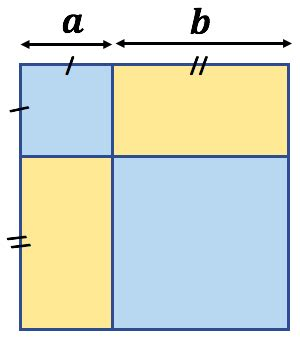
\includegraphics[width=3cm]{img/carredunesomme.jpg}
  \end{enumerate}
\end{exercise}

\begin{exercise}
  \parbox[t]{.45\linewidth}{Calcule l'aire et le périmètre de la partie grisée dans la figure ci-dessous. Veille à ce que tes expressions soient les plus réduites possible.
  }
  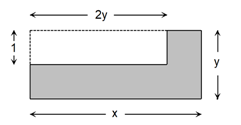
\includegraphics[valign=t]{img/aireetperi.png}
\end{exercise}

\begin{exercise}
  Calcule le volume et l'aire totale des faces de ce parallélipipède rectangle en te basant sur les informations données. Veille à ce que tes expressions finales soient les plus réduites possibles.
  \begin{center}
    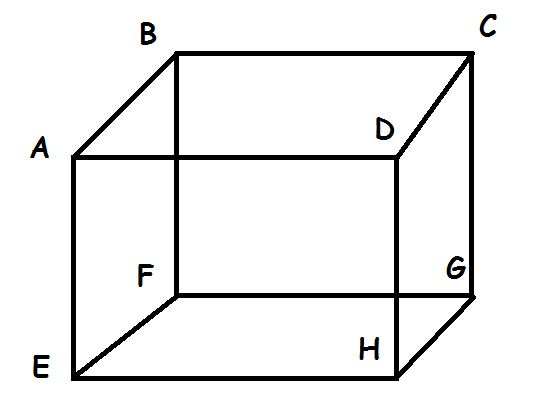
\includegraphics[width=6cm, valign=c]{img/parall.jpg}
    \parbox{5cm}{
      $|AB| = x + 2$\\
      $|GC| = 9 - x$\\
      $|AD| = 1 + 2x$
    }
     
  \end{center}  
\end{exercise}

\begin{exercise}
  Vrai ou faux? Justifie dans tous les cas.
  \begin{enumerate}
    \item Le carré d'un produit de deux facteurs est égal au produit des carrés de ces deux facteurs.
    \item Le carré d'une somme de deux termes est égal à la somme des carrés de ces deux termes.
    \item $13\cdot 28=\left(10\cdot 20\right) + \left(3\cdot 8\right)$
    \item $\left(3x+2y\right)^2=196$ si $x=2$ et $y=-1$
    \item $(3m + 2)^2=6m^2+4$
    \item $a-(3+c)=a-3+c$
  \end{enumerate}
\end{exercise}

\begin{exercise}
  Soit un carré dont le périmètre vaut $4\cdot \left(2x+3y\right)$. Détermine les expressions réduites qui représentent \dots
  \begin{enumerate}
    \item le côté du carré
    \item le périmètre du carré sous la forme d'une somme
    \item l'aire du carré (sous forme d'un produit)
    \item l'aire du carré (sous forme d'une somme)
  \end{enumerate}
\end{exercise}

\newpage

\begin{exercise}
  Voici deux figures. Pour chacune d'entre elles, calcule le périmètre et l'aire. Réduis au maximum les expressions obtenues.
  \begin{center}
    
\includegraphics[valign=t]{chapitres/calcul-litteral/img/fig.1.png}
    \hfil
    
\includegraphics[valign=t]{chapitres/calcul-litteral/img/fig.2.png}
  \end{center}
\end{exercise}

\begin{exercise}
  Calcule l'aire de la partie colorée en gris foncé des figures suivantes.
  \begin{center}
    
\includegraphics[width=16cm]{chapitres/calcul-litteral/img/airecoloree.PNG} 
  \end{center}
\end{exercise}

\newpage

\begin{exercise}
  \emph{(En dépassement)} Réduis les expressions suivantes au maximum. Fais attention à la priorité des opérations.
\newline
  Série 1
  \begin{enumerate}[itemsep=0.5cm]
    \item $-(-3+5a\cdot(-2)+6)-(+2a\cdot(-5))-13$
    \item $(15a+1)\cdot2+6-(3a-2-(5+a))$
    \item $3ab+5a\cdot(3b-2)-(-6a\cdot b)+77:11$
  \end{enumerate}
  \vspace{0.5cm}
  Série 2
  \begin{enumerate}[itemsep=0.5cm]
    \item $7a^2b-5b+(2-6a^2\cdot3b+2\cdot(-8b))$
    \item $-(3a+5a^2)-7a\cdot a+12a :(-6)$
    \item $5a-7\cdot (-a)+4\cdot(2a-6)+3$
  \end{enumerate}
  \vspace{0.5cm}
  Série 3
  \begin{enumerate}[itemsep=0.5cm]
    \item $-5xy+7x\cdot(-3y-2x)+4x\cdot 3x$
    \item $75\cdot(a-b)-15a-6a:(-2)$
    \item $6bc-(a\cdot(2b+c)-c\c(3a-5b))$
  \end{enumerate}
  \vspace{0.5cm}
\end{exercise}

\begin{exercise}
  \emph{(En dépassement)} Effectue les distributivités suivantes et respecte bien les formules des puissances ($a,b,c,x$ sont non nuls). 
  \newline
  Série 1
  \begin{enumerate}[cols=2]
    \item $(x^3+x^2x^0)\cdot(x^5y^7-y^3)$
    \item $(-a^{12}b^9-x^5)\cdot(a^6-b^{11})$
    \item $(x^0+y^3)\cdot(-a^2x^5+x^6y^9)$
    \item $\left(\dfrac{ac}{xb}+\dfrac{-x}{ab}\right)\cdot\left(\dfrac{x}{bc}-\dfrac{ax}{a}\right)$
    \item $\left(\dfrac{-a^8}{c^5}-\dfrac{x^7}{b^{10}}\right)\cdot\left(\dfrac{-c^4}{a^3}+\dfrac{b^8}{x^2}\right)$
    \item $-7\left(4a - 6a^3\right)$
  \end{enumerate}
  Série 2
  \begin{enumerate}[cols=2]
    \item $(-5^6+2x^3)\cdot(-7x^8+3a^2x^3)$
    \item $(4x^5-6x^2y^5)\cdot(-6x^2y^3)$
    \item $(-4x^7y^3-x)\cdot(5y^8+x^4)$
    \item $\left(\dfrac{x^7}{a^8b^4}+\dfrac{a^3}{c^6}\right)\cdot\left(\dfrac{c^7}{x^4}-\dfrac{c^3b^3}{a^5}\right)$
    \item $\left(\dfrac{a^7b^8}{x^5}-\dfrac{a^2}{b^7x^4}\right)\cdot\left(\dfrac{c^6x^4}{a^6}+\dfrac{b^5}{a^7}\right)$
    \item $\dfrac{4a+2b^2}{2}\cdot (-3ab)$
  \end{enumerate}
\end{exercise}

\end{document}